%--------------------------------------------------------------------------
% Paquetes y estilo del libro. http://www.tec-digital.itcr.ac.cr/revistamatematica/
% Versión Juio-2014
%--------------------------------------------------------------------------
% Paquetes 

\usepackage[english,spanish,es-tabla]{babel}
%\usepackage[latin1]{inputenc}                      % Entrada de acentos

\usepackage[spanish]{babel}                      % Entrada de acentos
\usepackage[utf8]{inputenc}

%---------------------------------------------------------------------------
% Para escribir codigo fuente java
\usepackage{listings}                      
% Definiendo colores
\usepackage{xcolor}
\definecolor{verde}{rgb}{0.25,0.5,0.35}
\definecolor{jpurple}{rgb}{0.5,0,0.35}

\usepackage{listings}
\lstset{
  language=Java,
  basicstyle=\ttfamily\small, 
  keywordstyle=\color{jpurple}\bfseries,
  stringstyle=\color{red},
  commentstyle=\color{verde},
  morecomment=[s][\color{blue}]{/**}{*/},
  extendedchars=true, 
  showspaces=false, 
  showstringspaces=false, 
  numbers=left,
  numberstyle=\tiny,
  breaklines=true, 
  backgroundcolor=\color{cyan!10}, 
  breakautoindent=true, 
  captionpos=b,
  xleftmargin=0pt,
  tabsize=4
}

\usepackage[T1]{fontenc}
\usepackage[autostyle, spanish = mexican]{csquotes}% manejo de comillas: " "
\MakeOuterQuote{"}
\usepackage{pslatex}                              % Fuentes finas postscript
%\usepackage[sc]{mathpazo}                         % Fuentes mathpazo
\usepackage{helvet}
\linespread{1.05}                                  % Fuente Palatino necesita espaciado
\usepackage[full]{textcomp}                        % Caracteres especiales como ' (recto)
\usepackage{xcolor}                                % Color: X11names (en el documentclass)
% COLORES personales---------------------------------------------------
    \definecolor{colortitulo}{RGB}{11,17,79} % 
    \definecolor{colordominante}{RGB}{11,17,79}
    \definecolor{colordominanteA}{RGB}{243,102,25}
    \definecolor{colordominanteF}{RGB}{219,68,14}
    \definecolor{colordominanteD}{RGB}{74,0,148}
   
    \definecolor{wcolornotas}{RGB}{74,0,148}%{RGB}{51,145,147} % 
    \definecolor{mostaza}{RGB}{231,196,25}
    \definecolor{amarilloM}{RGB}{248,199,90}
    \definecolor{amarilloD}{RGB}{251,237,121}
    \definecolor{azulF}{rgb}{.0,.0,.3}
    \definecolor{grisD}{rgb}{.3,.3,.3}
    \definecolor{grisF}{rgb}{.6,.6,.6}
    \definecolor{grisamarillo}{RGB}{248,248,245} 
    \definecolor{miverde}{RGB}{44,162,67}
    \definecolor{verdep}{RGB}{166,206,58}
    \definecolor{verdeF}{RGB}{5,92,8}
    \colorlet{mygray}{black!20}
    \newcommand{\verde}{\color{miverde}}
    \newcommand{\colornotas}{\color{wcolornotas}}
% Fin COLORES personales-------------------------------------------------
\usepackage{psboxit}
\usepackage{pstricks}
\usepackage{xparse}

\usepackage{tikz,tkz-tab}% Cajas de Teoremas, ejemplos, etc.
%listings para código en color en tcbcolor
\usetikzlibrary{matrix,arrows,
positioning,shadows,shadings,backgrounds,calc, shapes, tikzmark}%
\usepackage{tcolorbox, empheq} 
 % Librerías tcolorbox
\tcbuselibrary{skins,breakable,listings,theorems} 

\usepackage{xargs}                                 % Comandos con opciones
\DeclareGraphicsExtensions{.pdf,.png,.jpg}
\usepackage{multicol}
% %\usepackage{epstopdf}% Conversión - Miktes 2.9 o inferior, TexLive 2009. o inferior
\usepackage[small,bf,labelsep=period]{caption}
\usepackage[breaklinks,colorlinks=true, pdfstartview=FitV, linkcolor=azulF, citecolor=azulF, urlcolor=azulF]{hyperref}
\usepackage{amsmath,amssymb,amsfonts,latexsym,cancel,stmaryrd}%
\usepackage[ruled,,vlined,lined,linesnumbered,algochapter]{algorithm2e}
\usepackage{framed}
\usepackage{titletoc}
\usepackage{calc}
\usepackage{longtable} 
\usepackage{colortbl} 
\usepackage{tabularx}
\usepackage{fancyvrb}
%\usepackage{minted}   %habilitar solo en Ubuntu (Linux)
\usepackage{array}
\usepackage{wasysym}
\usepackage{supertabular}
\definecolor{verbmentsbgcolor}{rgb}{0.9764, 0.9764, 0.9762}
\definecolor{verbmentscaptionbgcolor}{rgb}{0.1647, 0.4980, 1}
\usepackage{verbments}
\fvset{frame=bottomline,framerule=0.01cm}
\plset{language=java,texcl=true,style=vs,%
listingnamefont=\sffamily\bfseries\color{white},%
bgcolor=verbmentsbgcolor,captionfont=\sffamily\color{white},%
captionbgcolor=verbmentscaptionbgcolor, listingname=\textbf{Programa}}
%\usepackage{pagecolor}
\usepackage[textwidth=2cm]{todonotes} 
\usepackage{booktabs}
\usepackage{marginnote}
\usepackage[b]{esvect}
\usepackage{rotating}
%\usepackage{float}
\usepackage{floatrow}
\usepackage[shortlabels]{enumitem}
\usepackage{subfigure}
\usepackage{wrapfig}
\usepackage{floatflt}
 \usepackage{kantlipsum} %\kant[1-13]


%----------------------------------------------------------------------------------------
% Fuentes especiales
%----------------------------------------------------------------------------------------
% Comandos para fuentes especiales
\newcommandx*{\fnte}[4][1=pag,2=9,3=n]{{\color{azulF}\fontfamily{#1}\fontseries{b}
\fontsize{#2}{1}\fontshape{#3}\selectfont{#4}}}

\newcommandx*{\fntb}[4][1=pag,2=9,3=n]{{\color{azulF}\fontfamily{#1}\fontsize{#2}{1}\fontseries{b}\fontshape{#3}\selectfont{#4}}}

\newcommandx*{\fntg}[4][1=pag,2=9,3=n]{{\color{grisF}\fontfamily{#1}\fontsize{#2}{1}\fontshape{#3}\selectfont{#4}}}

\newcommand{\fhv}[2]{{\fontfamily{pag}\fontsize{#1}{1}\selectfont{#2}}}

\newcommand{\fhvb}[2]{{\fontfamily{pag}\fontseries{b}\fontsize{#1}{1}\selectfont{#2}}}

% fontfamily %n = normal, it =italics
\newcommandx*{\fntl}[4][1=pag,2=10,3=n]{{\colornotas\fontfamily{#1}\fontsize{#2}{1}\fontseries{b}\fontshape{#3}\selectfont{#4}}}

\newcommandx*{\tfntl}[4][1=pag,2=10,3=n]{{\color{azulF}\fontfamily{#1}\fontsize{#2}{1}\fontseries{b}\fontshape{#3}\selectfont{#4}}}

\newcommandx*{\fnt}[4][1=pag,2=9,3=n]{{\colornotas\fontfamily{#1}\fontsize{#2}{1}\fontshape{#3}\selectfont{#4}}}

\newcommandx*{\colrfnt}[4][1=pag,2=9,3=n]{{\red\fontfamily{#1}\fontsize{#2}{1}\fontshape{#3}\selectfont{#4}}}

\newcommandx*{\nfnt}[4][1=pag,2=9,3=n]{{\fontfamily{#1}\fontsize{#2}{1}\fontshape{#3}\selectfont{#4}}}

\newcommand{\wfont}[2]{{\fontfamily{#1}\selectfont{#2}}}
\newcommand{\fptm}[1]{{\fontfamily{ptm}\selectfont{#1}}}

\newcommandx*{\cfnte}[4][1=pag,2=9,3=n]{{\wcelestetxt\fontfamily{#1}\fontsize{#2}{1}\fontshape{#3}\selectfont{#4}}}
% Fin fuentes----------------------------------------------------------

%----------------------------------------------------------------------------------------
% Cabeceras
%----------------------------------------------------------------------------------------
% Elimina el encabezado de las páginas impares vacías al final de los capítulos
\makeatletter
\renewcommand{\cleardoublepage}{
\clearpage\ifodd\c@page\else
\hbox{}
\vspace*{\fill}
\thispagestyle{empty}
\newpage
\fi}
\makeatother

\usepackage{fancyhdr}
% Números de página en rectángulos y capítulo. Necesitamos posicionar los nodos
\usepackage[absolute]{textpos}
    \setlength{\TPHorizModule}{10mm}% 1 generic horizontal unit is equivalent to 10mm
    \setlength{\TPVertModule}{10mm}% 1 generic vertical unit is equivalent to 10mm
    \textblockorigin{0mm}{0mm}% top left corner set as origin

\makeatletter
% Redefinir \chaptermark sin "capítulo" ni número de capítulo, solo el texto.
\renewcommand{\chaptermark}[1]{\markboth{\if@mainmatter\ ~~\fi#1}{}}
\makeatother

%------------------------------------------------------------------------------
% Decoración de cabeceras 
% Texto en secciones
\renewcommand{\sectionmark}[1]{\markright{\sffamily\normalsize\thesection\hspace{5pt}#1}{}} 
% Configuración de fuentes para el número de página en el encabezado
\fancyhf{} 
% > OP 1: Todas las páginas con la sección a la izquierda
%   \fancyhead[LO,LE]{\rightmark} % L=Left, O=Odd y  E=Even pages
% > OP 2: Todas las páginas con la seción a la izquierda en un rectángulo (todo el header)
%   \usepackage{tikzpagenodes}
%   \fancyhead[LO,LE]{\rightmark
%   \begin{textblock}{1}(0,0)
%   \begin{tikzpicture}[remember picture,overlay]
%   \fill[grisamarillo] (current page.north west) 
%     rectangle
%   ([xshift=2pt,yshift=-3pt]current page.east|-current page header area.south east);
%   \end{tikzpicture}
%   \end{textblock}
%   }
% > OP 3: Todas las páginas con la seción a la izquierda en rectángulo bordes difusos
\usepackage{tikzpagenodes}
\usetikzlibrary{decorations.pathmorphing,calc,shadows.blur,shadings}
\pgfmathsetseed{1}

\pgfdeclaredecoration{irregular fractal line}{init}
{
  \state{init}[width=\pgfdecoratedinputsegmentremainingdistance]
  {
    \pgfpathlineto{\pgfpoint{random*\pgfdecoratedinputsegmentremainingdistance}{(random*\pgfdecorationsegmentamplitude-0.02)*\pgfdecoratedinputsegmentremainingdistance}}
    \pgfpathlineto{\pgfpoint{\pgfdecoratedinputsegmentremainingdistance}{0pt}}
  }
}

\tikzset{
   paper/.style={draw=black!10, blur shadow, shade=bilinear interpolation,
                 lower left=black!20, upper left=black!15, upper right=white, lower right=black!10},
   irregular border/.style={decoration={irregular fractal line, amplitude=0.2},
           decorate,
     },
   ragged border/.style={ decoration={random steps, segment length=7mm, amplitude=2mm},
           decorate,
   }
}
%L=Left, Odd Even - Decoración en encabezado
\fancyhead[LO,LE]{\rightmark {\color{grisF}
  \href{http://www.tec-digital.itcr.ac.cr/revistamatematica/}{\sffamily\normalsize   \;(http://www.tec-digital.itcr.ac.cr/revistamatematica/).}}
\begin{textblock}{1}(0,0)
\begin{tikzpicture}[remember picture,overlay]
  \fill[verdep,opacity=0.7]
        decorate[irregular border]{decorate{decorate{decorate{decorate[ragged border]{
        ($(current page header area.south east-|current page.east) - (0, random*5mm)$) -- ($(current page header area.south west-|current page.west) - (0, random*5mm)$)
        }}}}}
        -- (current page.north west) -- (current page.north east) -- cycle;
\end{tikzpicture}
\end{textblock}
}
% Fin decoración cabeceras
\renewcommand{\headrulewidth}{0pt}   % Ancho de la línea bajo el encabezado
\addtolength{\headheight}{2.5pt}     % Aumente el espacio alrededor de la cabecera 
\renewcommand{\footrulewidth}{0pt}   % Elimina la línea en el pie de página
% Estilo para  "pagestyle plain"
\fancypagestyle{plain}{\fancyhead{}\renewcommand{\headrulewidth}{0pt}} 



% Números de página+chaptertitle en rectángulo en el borde
\fancyfoot[LE]{
\begin{textblock}{3}(21,5)
\begin{tikzpicture}[overlay]
\node[draw=colordominante,
rectangle,minimum width=2cm, minimum height=2cm,
anchor=west,
fill=colordominante,font=\fontsize{25}{1}\sffamily\bfseries,inner sep=2pt,outer sep=2pt] 
at (-1.5cm,0pt){\textcolor{gray!10}{\thepage}};
%cap
\node[right,line width=1pt,rectangle,
fill=grisamarillo,font=\fontsize{35}{1}\sffamily\bfseries,inner sep=20pt,outer sep=60pt,
rotate=-90] at (current page.south west){\textcolor{gray!30}{\leftmark}};  
\end{tikzpicture}
\end{textblock}
}

\fancyfoot[RO]{
\begin{textblock}{3}(18,5)
\begin{tikzpicture}[overlay]
\node[draw=colordominante,rectangle,minimum width=2cm, minimum height=2cm,
anchor=west,
fill=colordominante,font=\fontsize{25}{1}\sffamily\bfseries,inner sep=2pt,outer sep=2pt] 
at (-1.5cm,0pt){\textcolor{gray!10}{\thepage}};
% %cap
% \node[left,line width=1pt,rectangle,
% fill=grisamarillo,font=\fontsize{35}{1}\sffamily\bfseries,inner sep=20pt,outer sep=60pt,
% rotate=90]at (current page.south west){\textcolor{gray!30}{\leftmark}};    
\end{tikzpicture}
\end{textblock}
}
\setlength\headheight{14.5pt} % 
% Fin cabeceras 

%----------------------------------------------------------------------------------------
% Color en los márgenes
%----------------------------------------------------------------------------------------
% \pagecolor{grisamarillo}
% \usepackage{eso-pic}
% \pagecolor{grisamarillo}
% \AddToShipoutPictureBG{%
%  \AtTextLowerLeft{\color{grisamarillo}%
%   \rule[-\footskip]{\textwidth}{\dimexpr\textheight+\footskip}}}

% Fin color márgenes


%----------------------------------------------------------------------------------------
% Prólogo
%----------------------------------------------------------------------------------------
\NewDocumentEnvironment{prologo}{O{}}{%
\chapter*{Prólogo}
\addcontentsline{toc}{schapter}{\addvspace{30pt}\large\sc\bfseries Prólogo \hfill \color{azulF}  }
\smallskip\smallskip
\begin{minipage}{0.9\textwidth}
 #1}{\end{minipage}}
 

%----------------------------------------------------------------------------------------
% Título
%----------------------------------------------------------------------------------------
\newcommand*{\titulo}[4]{\begingroup%
\raggedleft 
\vspace*{\baselineskip} % Espacio en blanco en la parte superior de la página
{\Large #1}\\[0.167\textheight] % Autor
{\LARGE\bfseries #2}\\[\baselineskip] % pre-título
{\textcolor{colortitulo}{\Huge #3}}\\[\baselineskip] % Título
{\Large \textit{#4}}\par % Descripción adicional

\vfill % Espacio en blanco entre el bloque de título y "la editorial"

{\raggedright
\begin{minipage}[c]{0.08\textwidth}
\raisebox{-2.0cm}{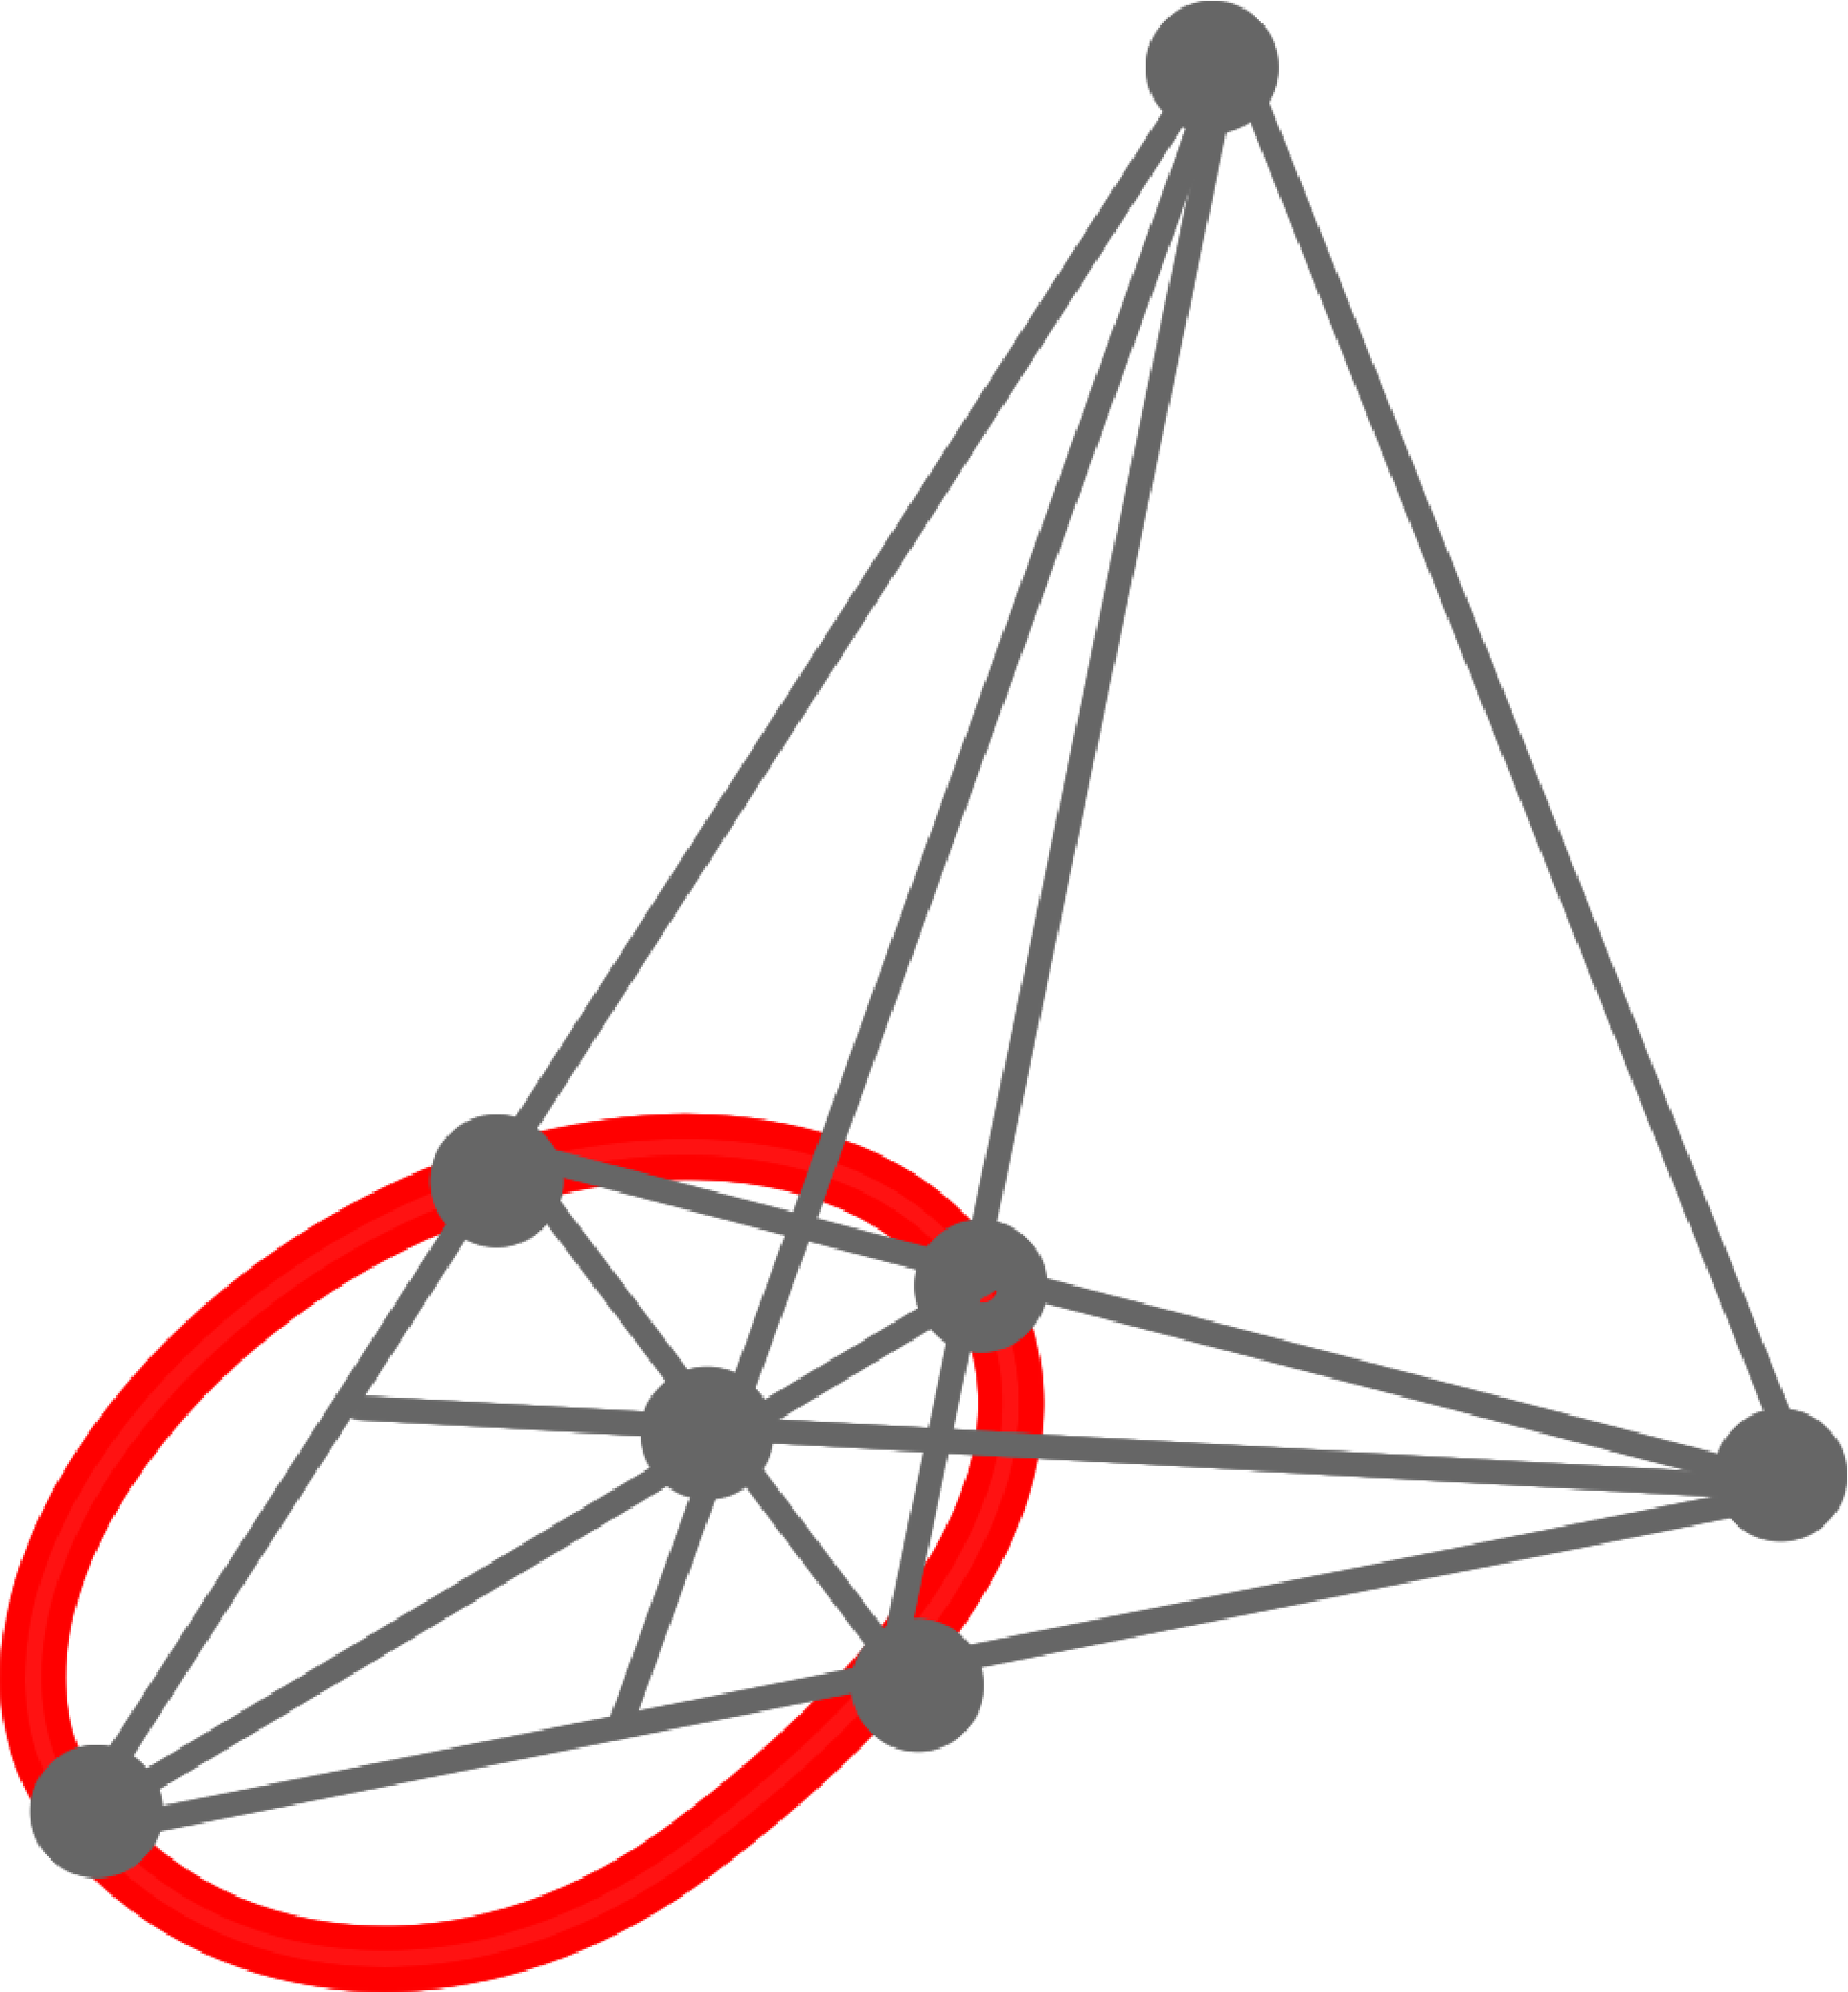
\includegraphics[width=1.4cm]{images/logo}}
 \end{minipage}
\  \ \hfill\begin{minipage}[t]{0.9\textwidth}
{\color{gray}
 \fhv{9}{Revista digital}\\
 \fhvb{9}{\color{azulF}Matemática, Educación e Internet.}
  \fntg[pag][8]{\color{grisF}
  \href{http://www.tec-digital.itcr.ac.cr/revistamatematica/}{(http://www.tec-digital.itcr.ac.cr/revistamatematica/).}}}
\end{minipage}          
}%raggedright
\vspace*{3\baselineskip} % Espacio en blanco antes del final de página
\endgroup}
% Fin Titulo--------------------------------------------------------


%----------------------------------------------------------------------------------------
% Copypright, ISBN, ...
%----------------------------------------------------------------------------------------
\def\copyrightpage{\thispagestyle{empty}%
\vbox to\textheight\bgroup\vfill\obeylines\obeyspaces\xcopyrightpage}

\def\xcopyrightpage#1#2\end#3{\scriptsize\parindent=0pt
Copyright\copyright{#1} 
\vskip40pt
#2\vskip200pt\egroup\endgroup}
\let\endcopyrightpage\relax


%Imprimir info  al pie de página
\makeatletter 
\newif\ifoffprintinfo
\def\dooffprintinfo{\global\offprintinfotrue}

\def\copyrightyear#1{\def\thecopyrightyear{#1}}

\copyrightyear{\the\year}

\def\dofnote#1#2{\vtop{\hyphenpenalty=10000
\advance\hsize -10pt \raggedright
\footnotesize{\it #1. }{ #2}\\
\noindent\hbox{\footnotesize
Derechos Reservados \copyright\ \thecopyrightyear\ Revista digital Matem\'atica, Educaci\'on e Internet
 ({\scriptsize\tt www.tec-digital.itcr.ac.cr/revistamatematica/)}}}}

\def\offprintinfo#1#2{
\def\theoffprint{\bgroup\frenchspacing
\dofnote{#1}{#2}
\egroup}}

\def\x@makefntext#1{
\kern-3\p@
\hrule\@width.4\columnwidth
\kern2.6\p@
\vrule height 9pt width0pt \relax
#1}

\def\offprintinfoerror{\typeout{^^J^^J
!! Debe poner {\string\offprintinfo\string{(Title,
Edition)\string}\string{(Author)\string}^^J en el inicio del documento.!!^^J^^J}}
\bgroup
\x@makefntext{Debe poner {\tt \string\offprintinfo\string{(Title,
Edition)\string}\string{(Author)\string}\newline en el inicio del documento.\vrule depth8pt width0pt}\egroup}}


\def\printoffprintinfo{\vtop to0pt{%
\hsize=\textwidth\footnotesize
\expandafter\ifx\csname theoffprint\endcsname\relax
\offprintinfoerror\else\theoffprint\fi\vskip1sp\vss}}


\def\@xfootnote[#1]{%
  \protected@xdef\@thefnmark{#1}%
  \@footnotemark\@footnotetext}
\makeatother

% Uso: \inforevista{Edición de Textos Científicos con LaTeX}{Walter Mora F., Alex Borbón A.}
\newcommand{\inforevista}{\protect\footnote[ ]{\printoffprintinfo}}


% Fin Copyright

%----------------------------------------------------------------------------------------
% CONTENIDO 
%----------------------------------------------------------------------------------------

%\usepackage{titletoc}
\contentsmargin{0cm}
\titlecontents{chapter}[0pc]
{\addvspace{30pt}%
  \begin{tikzpicture}[remember picture, overlay]%
  \draw[fill=verdep!70,draw=verdep!70] (-4,-.1) rectangle (-0.1,0.5);%
  \pgftext[left,x=-1.5 cm,y=0.2cm]{\color{azulF}\Huge\sc\bfseries \thecontentslabel};%
  \end{tikzpicture}\color{azulF}\large\sc\bfseries%
}%
{}
{}
%{\;\color{verdep!70}\titlerule\;\color{azulF}\large\sc\bfseries Página \thecontentspage
{\;\color{verdep!70}\titlerule\;\color{azulF}\large\sc\bfseries \thecontentspage
\begin{tikzpicture}[remember picture, overlay]
\draw[fill=verdep!70,draw=verdep!70] (1pt,0) rectangle (6,0.1pt);
\end{tikzpicture}}%

\titlecontents{section}[2.4pc]
{\addvspace{1pt}}
{\contentslabel[\color{azulF}\thecontentslabel]{2.4pc}}
{}
{\hfill\small \color{azulF}\thecontentspage}
[]
\titlecontents*{subsection}[4pc]
{\addvspace{-1pt}\small}
{}
{}
{\hfill\small \color{azulF}\thecontentspage}
[\\][]

\makeatletter
\renewcommand{\tableofcontents}{%
\chapter*{%
\vspace*{-20\p@}%
\begin{tikzpicture}[remember picture, overlay]%
\pgftext[right,x=15cm,y=0.2cm]{\color{azulF}\Huge\sc\bfseries \contentsname};%
\draw[fill=verdep!70,draw=verdep!70] (13,-1) rectangle (20,1.75);%
\clip (13,-1) rectangle (20,1.75);
%\pgftext[right,x=15cm,y=0.2cm]{\color{white}\Huge\sc\bfseries \contentsname};%
\pgftext[right,x=15cm,y=0.2cm]{\color{azulF}\Huge\sc\bfseries \contentsname};%
\end{tikzpicture}}%
\@starttoc{toc}}
\makeatother
% Fin Contenido 

%----------------------------------------------------------------------------------------
% CAPITULO Estilo simple
%----------------------------------------------------------------------------------------

\usepackage{titlesec}
\newcommand{\hsp}{\hspace{15pt}}
\titleformat{\chapter}[hang]{\huge\bfseries}{{
        \fontsize{6em}{6em}\selectfont\black
        \thechapter}\hsp\textcolor{verdep}{\vrule height 4em width 2pt}\hsp}{0pt}{\huge\bfseries}
% Subir el título
%\titlespacing*{\chapter}{0cm}{-\topskip}{0pt}[0pt]        


%----------------------------------------------------------------------------------------
%	Numeración de las secciones -- en el margen
%----------------------------------------------------------------------------------------

\makeatletter
\renewcommand{\@seccntformat}[1]{\llap{\textcolor{verdeF}{\csname the#1\endcsname}\hspace{1em}}}                    
\renewcommand{\section}{\@startsection{section}{1}{\z@}
{-4ex \@plus -1ex \@minus -.4ex}
{1ex \@plus.2ex }
{\color{azulF}\normalfont\huge\sffamily\bfseries}}
\renewcommand{\subsection}{\@startsection {subsection}{2}{\z@}
{-3ex \@plus -0.1ex \@minus -.4ex}
{0.5ex \@plus.2ex }
{\normalfont\sffamily\bfseries}}
\renewcommand{\subsubsection}{\@startsection {subsubsection}{3}{\z@}
{-2ex \@plus -0.1ex \@minus -.2ex}
{0.2ex \@plus.2ex }
{\normalfont\small\sffamily\bfseries}}                        
\renewcommand\paragraph{\@startsection{paragraph}{4}{\z@}
{-2ex \@plus-.2ex \@minus .2ex}
{0.1ex}
{\normalfont\small\sffamily\bfseries}}
\makeatother
% Fin numeración secciones



%---------------------------------------------------------------------------------
%  Entornos:  Ejemplo, teorema, proposición, lema, lista de ejercicios, 
%             caja interludio, caja simple  
%---------------------------------------------------------------------------------

%  Cajas con el paquete  tcbcolor
%  CONTADORES: ejemplo, definicion, lema, teorema, corolario, proposicion,ejercicio 
\newcounter{tcbteo}[chapter]
\renewcommand{\thetcbteo}{\thechapter.\arabic{tcbteo}}

\newcounter{tcbdefi}[chapter]
\renewcommand{\thetcbdefi}{\thechapter.\arabic{tcbdefi}}

\newcounter{tcblema}[chapter]
\renewcommand{\thetcblema}{\thechapter.\arabic{tcblema}}

\newcounter{tcbcoro}[chapter]
\renewcommand{\thetcbcoro}{\thechapter.\arabic{tcbcoro}}

%  \newcounter{tcbListaEjercicios}[chapter]
%  \renewcommand{\thetcbListaEjercicios}{\thechapter.\arabic{tcbListaEjercicios}}

\newcounter{tcbpropo}[chapter]
\renewcommand{\thetcbpropo}{\thechapter.\arabic{tcbpropo}}

\newlength{\examlen}
\tikzset{
    wnodeTeorema/.style={%
         rectangle,  top color=gray!5, bottom color=gray!5,
         inner sep=1mm,anchor=west,font=\small\bf\sffamily},
   wnodeminimo/.style={%
         rectangle,  top color=white, bottom color=white,
         text=azulF,inner sep=1mm,anchor=west,font=\small\bf\sffamily}      
}



%\begin{teorema}  o \begin{teorema}[de tal] o \begin{teorema}[][ref]
% Teorema -----------------------------------------------------
\newtcolorbox{wwteorema}[3][]{%
arc=0mm,breakable,enhanced,colback=gray!5,boxrule=0pt,top=7mm,
drop fuzzy shadow,
fontupper=\normalsize,step and label={tcbteo}{#3},
% Caso normal, sin quiebres
overlay unbroken ={%
\draw[color=colordominanteD,line width=0.2pt] (frame.north west)--([xshift=0pt]frame.north east);
%Caja de Título: teo --
\node[wnodeTeorema](tituloteo) at ([xshift=0pt, yshift=-4mm]frame.north west)
{\textbf{\color{colordominanteD} Teorema \thetcbteo \;#2}};
%Borde superior --
\draw[colordominanteD,line width=2.5cm] ([xshift=1.25cm, yshift=0cm]frame.north west)-- +(\examlen,3pt);
},
% Caso de quiebre por cambio de página
overlay first = {%
\draw[color=colordominanteD,line width=0.2pt] (frame.north west)--([xshift=0pt]frame.north east);
%Caja de Título: teo --
\node[wnodeTeorema](tituloteo) at ([xshift=0pt, yshift=-4mm]frame.north west)
{\textbf{\color{colordominanteD} Teorema \thetcbteo \;#2}};
%Borde superior --
\draw[colordominanteD,line width=2.5cm] ([xshift=1.25cm, yshift=0cm]frame.north west)-- +(\examlen,3pt);
                }, 
overlay middle={},                
% Mantener borde en cambio de página 
overlay last = {\draw[color=colordominanteD,line width=0.2pt] (frame.north west)--([xshift=0pt]frame.north east);
                } 
#1}
%-
\NewDocumentEnvironment{teorema}{O{} O{} O{}}{\smallskip\begin{wwteorema}{#1}{#2}%
 #3}{\end{wwteorema}\smallskip }
% TEOREMA---------------------------------------------------------



%\begin{proposicion}  o \begin{proposicion}[de tal] o \begin{proposicion}[][ref]
% Proposición-----------------------------------------------------
\newtcolorbox{wwpropo}[3][]{%
arc=0mm,breakable,enhanced,colback=gray!5,boxrule=0pt,top=7mm,
fontupper=\normalsize,step and label={tcbpropo}{#3},
% Caso normal, sin quiebres
overlay unbroken ={%
\draw[color=colordominante,line width=0.2pt] (frame.north west)--([xshift=0pt]frame.north east);        
%Caja de Título: propo --
\node[wnodeTeorema](tituloteo) at ([xshift=0pt, yshift=-4mm]frame.north west)
{\textbf{\color{colordominante} Proposición \thetcbpropo\;#2}};
%Borde superior --
\draw[colordominante,line width=2.5cm] ([xshift=1.25cm, yshift=0cm]frame.north west)-- +(\examlen,3pt);
%barra vertical
\draw[color=gray,line width=3pt] ([xshift=2pt] frame.north west)--([xshift=2pt] frame.south west);
},
overlay first ={%
\draw[color=colordominante,line width=0.2pt] (frame.north west)--([xshift=0pt]frame.north east);        
%Caja de Título: propo --
\node[wnodeTeorema](tituloteo) at ([xshift=0pt, yshift=-4mm]frame.north west)
{\textbf{\color{colordominante} Proposición \thetcbpropo\;#2}};
%Borde superior --
\draw[colordominante,line width=2.5cm] ([xshift=1.25cm, yshift=0cm]frame.north west)-- +(\examlen,3pt);
}, %
overlay middle={%barra vertical
\draw[color=gray,line width=3pt] ([xshift=2pt] frame.north west)--([xshift=2pt] frame.south west);},
% Mantener borde en cambio de página 
overlay last ={\draw[color=colordominante,line width=0.2pt] (frame.north west)--([xshift=0pt]frame.north east);
        }
#1}
%-
\NewDocumentEnvironment{proposicion}{O{} O{} O{}}{\smallskip\begin{wwpropo}{#1}{#2}%
 #3}{\end{wwpropo}\smallskip }
% ---------------------------------------------------------



% LEMA -----------------------------------------------------------
 \newtcolorbox{wwlema}[3][]{%
arc=0mm,breakable,enhanced,colback=gray!5,boxrule=0pt,
top=1mm, left=3pt,
step and label={tcblema}{#3},
fontupper={\small\bf\sffamily {\color{azulF}Lema \thetcblema \;#2}}~\normalfont, %"Lema..."+texto del cuerpo
overlay unbroken ={%
%barra vertical
\draw[color=gray,line width=3pt] ([xshift=2pt] frame.north west)--([xshift=2pt] frame.south west);
},
overlay first  = {%barra vertical
\draw[color=gray,line width=3pt] ([xshift=2pt] frame.north west)--([xshift=2pt] frame.south west);
},     
overlay middle={%barra vertical
\draw[color=gray,line width=3pt] ([xshift=2pt] frame.north west)--([xshift=2pt] frame.south west);}, 
% Mantener borde en cambio de página     
overlay last ={\draw[color=gray,line width=3pt] ([xshift=2pt] frame.north west)--([xshift=2pt] frame.south west);   }    
#1}
%-
\NewDocumentEnvironment{lema}{O{} O{} O{}}{\smallskip\begin{wwlema}{#1}{#2}%
#3}{\end{wwlema}\smallskip }
%LEMA--------------------------------------------------------------


% % Corolario -------------------------------------------------------
\newtcolorbox{wwcoro}[2][]{%
arc=0mm,breakable,enhanced,colback=gray!5,boxrule=0pt,
top=1mm,left=3pt,
fontupper={\small\bf\sffamily {\color{azulF}Corolario \thetcbcoro}\;}~\normalfont, 
step and label={tcbcoro}{#2},
overlay unbroken ={%
%barra vertical
\draw[color=gray,line width=3pt] ([xshift=2pt] frame.north west)--([xshift=2pt] frame.south west);  
},
overlay first  = {%barra vertical
\draw[color=gray,line width=3pt] ([xshift=2pt] frame.north west)--([xshift=2pt] frame.south west);                 
        },%
overlay middle={%barra vertical
\draw[color=gray,line width=3pt] ([xshift=2pt] frame.north west)--([xshift=2pt] frame.south west);},        
% Mantener borde en cambio de página     
overlay last ={\draw[color=gray,line width=3pt] 
                     ([xshift=2pt] frame.north west)--([xshift=2pt] frame.south west);
              }     
#1}
%-
\NewDocumentEnvironment{corolario}{O{} O{}}{\smallskip\begin{wwcoro}{#1}%
}{\end{wwcoro}\smallskip }
% Corolario------------------------------------------------------


% % Definición---------------------------------------------------
\newtcolorbox{wwdefinicion}[3][]{%
arc=0mm,breakable,enhanced,colback=gray!5,boxrule=0pt,drop fuzzy shadow,
top=6mm,fontupper=\normalsize,step and label={tcbdefi}{#3},
overlay unbroken ={%
%barra vertical
\draw[color=colordominanteA,line width=3pt] ([xshift=2pt] frame.north west)--([xshift=2pt] frame.south west);                           
%Caja de Título: defi --
\node[wnodeTeorema](titulodefi) at ([xshift=4.5pt, yshift=-3mm]frame.north west)
{\textbf{Definición \thetcbdefi \;#2}};
},
overlay first  = {
%barra vertical
\draw[color=colordominanteA,line width=3pt] ([xshift=2pt] frame.north west)--([xshift=2pt] frame.south west);                         
%Caja de Título: defi --
\node[wnodeTeorema](titulodefi) at ([xshift=4.5pt, yshift=-3mm]frame.north west)
{\textbf{Definición \thetcbdefi \;#2}};
                }, %overlay
% Mantener borde en cambio de página
overlay middle={%barra vertical
\draw[color=colordominanteA,line width=3pt] ([xshift=2pt] frame.north west)--([xshift=2pt] frame.south west); 
}, 
overlay last    = {%barra vertical
\draw[color=colordominanteA,line width=3pt] ([xshift=2pt] frame.north west)--([xshift=2pt] frame.south west);}
#1}
%-
\NewDocumentEnvironment{definicion}{O{} O{} O{}}{\smallskip\begin{wwdefinicion}{#1}{#2}%
 #3}{\end{wwdefinicion}\smallskip }
% %DEFINICION---------------------------------------------------------


% Caja para Ejemplo --------------------------------------------------
\newcounter{tcbejem}[chapter]
\renewcommand{\thetcbejem}{\thechapter.\arabic{tcbejem}}
\colorlet{colorfondoejemplo}{gray!5}
\definecolor{colorejemplo}{rgb}{.0,.0,.3}
% Ejemplo
\newtcolorbox{wwejemplo}[3][]{%
arc=0mm,
breakable,drop fuzzy shadow,
enhanced,
colback=grisamarillo,
boxrule=0pt,
top=8mm, %Separación vertical - inicia texto
enlarge top by=\baselineskip/2+1mm,
enlarge top at break by=0mm,pad at break=2mm,
fontupper=\normalsize,
step and label={tcbejem}{#3},
overlay unbroken={%barra vertical
\draw[color=verdep,line width=3pt] ([xshift=2pt] frame.north west)--([xshift=2pt] frame.south west);                            
% Caja de imagen Ejemplo
\node[rectangle, 
         text=black, 
         inner sep=1mm,anchor=west,font=\small\bf\sffamily] at ([xshift=-14.3pt,yshift=-4.1mm]frame.north west)%
{
\includegraphics{images/nodoejemplo}\raisebox{0.5cm}{}};
% Caja numeración y descripción
\node[rectangle, 
 text=black, 
 inner sep=1mm,
 anchor=west,
 font=\normalsize] at ([xshift=1.1cm,yshift=-2.9mm]frame.north west)%
 {\fhvb{10}{\;\thetcbejem \;\;\;#2}}; }, % overlay
overlay first  = {%
%barra vertical
\draw[color=verdep,line width=3pt] ([xshift=2pt] frame.north west)--([xshift=2pt] frame.south west);                            
% Caja de imagen Ejemplo
\node[rectangle, 
         text=black, 
         inner sep=1mm,anchor=west,font=\small\bf\sffamily] at ([xshift=-14.3pt,yshift=-4.1mm]frame.north west)%
{
\includegraphics{images/nodoejemplo}\raisebox{0.5cm}{}};
% Caja numeración y descripción
\node[rectangle, 
 text=black, 
 inner sep=1mm,
 anchor=west,
 font=\normalsize] at ([xshift=1.1cm,yshift=-2.9mm]frame.north west)%
 {\fhvb{10}{\;\thetcbejem \;\;\;#2}};
 },%overlay first    
%Borde cambio de páginas
overlay middle={%barra vertical
\draw[color=verdep,line width=3pt] ([xshift=2pt] frame.north west)--([xshift=2pt] frame.south west); },
overlay last={%barra vertical
\draw[color=verdep,line width=3pt] ([xshift=2pt] frame.north west)--([xshift=2pt] frame.south west); }
#1}
%-
\NewDocumentEnvironment{ejemplo}{O{} O{} O{}}{\smallskip\begin{wwejemplo}{#1}{#2}%
 #3}{\end{wwejemplo}\smallskip }
%EJEMPLO-----------------------------------------------------------------



% CAJA de comentario-----------------------------------------------------
\definecolor{colrnodocaja}{RGB}{44,91,144}
\definecolor{colrfondocaja}{RGB}{241,241,227}
%CAJA de comentario ------------------------------------------------------
\newtcolorbox{wwcaja}[2][]{%
arc=0mm,breakable,drop fuzzy shadow,
enhanced,colback=gray!4,
boxrule=0pt,
top=3mm, %Separación vertical - inicia texto
enlarge top by=\baselineskip/2+1mm,
enlarge top at break by=0mm,pad at break=2mm,
fontupper=\normalsize,
%step and label={tcbca}{#3},
overlay unbroken ={%
\draw[color=gray!2,line width=0.2pt] (frame.north west)
  --([xshift=0pt]frame.north east)
  --([xshift=0pt]frame.south east)
  --([xshift=0pt]frame.south west)--(frame.north west);
% Caja de Título CAJA
\node[ rectangle, %minimum width=0cm, minimum height=0.0cm,
         top color=amarilloD, bottom color=amarilloD,
         inner sep=0.5mm,anchor=west,font=\normalsize]at ([xshift=-0.5pt,  yshift=2.30mm]frame.north west){\fnte[pag][10]{ \bf #2}};
},
%Borde
overlay first={\draw[color=gray!2,line width=0.2pt] (frame.north west)
  --([xshift=0pt]frame.north east)
  --([xshift=0pt]frame.south east)
  --([xshift=0pt]frame.south west)--(frame.north west);
% Caja de Título CAJA
\node[ rectangle, %minimum width=0cm, minimum height=0.0cm,
         top color=amarilloD, bottom color=amarilloD,
         inner sep=0.5mm,anchor=west,font=\normalsize]at ([xshift=-0.5pt,  yshift=2.30mm]frame.north west){\fnte[pag][10]{ \bf #2}};
         },
overlay middle={},         
%Borde cambio de página
overlay last={\draw[color=gray!2,line width=0.2pt] (frame.north west)
  --([xshift=0pt]frame.north east)
  --([xshift=0pt]frame.south east)
  --([xshift=0pt]frame.south west)--(frame.north west);}
#1}
%-
\NewDocumentEnvironment{caja}{O{} O{}}{\smallskip\begin{wwcaja}{#1}%
 #2}{\end{wwcaja}\smallskip }
% CAJA de comentario

% Fin mis entornos---------------------------------------------------------------


%-----------------------------------------------------------------------------
% TABLAS CON Tikz
%----------------------------------------------------------------------------- 
\usepackage{array}
\usetikzlibrary{calc,fit,shadows,arrows,positioning}
\pgfdeclarelayer{background}
\pgfdeclarelayer{foreground}
\pgfsetlayers{background,main,foreground}
%--
%------------------------------------------------------------------------------
% Data Table
%------------------------------------------------------------------------------
\newsavebox{\dataTableContent} % Box
\newenvironment{dataTable}[1] % \new environment
{%
\begin{lrbox}{\dataTableContent}%
\begin{tabular}{#1}}%
%
{%
\end{tabular}
\end{lrbox}
\begin{tikzpicture}
\node [inner xsep=0pt] (tbl){\usebox{\dataTableContent}};
\begin{pgfonlayer}{background}
% table
\draw[rounded corners=1pt,top color=gray!1,bottom color=gray!30,draw=black]
(tbl.north east) rectangle (tbl.south west);
% top line
\draw[rounded corners=1pt,top color=gray!10!black,bottom color=gray!50!black,draw=black]%
($(tbl.north west)$) rectangle ($(tbl.north east)-(0,1.5\baselineskip)$);
% bottom rule
\draw[rounded corners=0.25pt,fill=gray,draw=black]%
(tbl.south west) rectangle ($(tbl.south east)+(0,0.05)$);
\end{pgfonlayer}
\end{tikzpicture}}
% --

  
 
 %---------------------------------------Matrices iluminadas------------------------
 %\usetikzlibrary{matrix,backgrounds}
\pgfdeclarelayer{wfondo}
\pgfsetlayers{wfondo,background,main}  
\NewDocumentCommand{\iluminar}{O{blue!40} m m}{%
\draw[#1, fill=#1] (#2.north west) rectangle (#3.south east);
}
% Ejemplos de entornos--------------------------------------------------------------




%----------------------------------------------------------------------------------------
%---------------------------------------------------------------------------------
%  Código de programas (LaTeX en ese caso) con Listings
%---------------------------------------------------------------------------------
% Listings
\usepackage{listings}% uso: \lstinline|section| y \begin{lstlisting}... \end{lstlisting}
\usepackage[scaled=0.83]{beramono} % para font \ttfamily en lstlisting
\lstset{ %
	      language={[LaTeX]TeX}, % lenguaje
	      basicstyle=\bfseries\ttfamily,
	      keywordstyle=\color{blue},
	      commentstyle=\color{brown},	   
	      backgroundcolor=\color{gray!15},
	      showstringspaces=false,
	      flexiblecolumns=true,
	      stringstyle=\ttfamily\color{blue},
	      extendedchars=true,	     
emph={rm,bf,it,sf,sl,sc,tt,gtrdot,lesseqqgtr,fcolorbox
      },     
emphstyle={\color{blue}\textbf}, % Color de caracteres especiales
literate=%
   *{$}{{{\color{red}\$}}}1
    {$$}{{{\color{red}\$\$}}}1
%No dejar líneas en blanco
}%fin lst
\newcommand{\wlatex}{\lstinline}


%CODIGO PARA EJEMPLOS-------------------------------------------------------


 % Ejemplo con \def
 \def\minorma(#1,#2,#3){\sqrt{#1^2+#2^2+#3^2}} 
 \def\lanorma#1{\minormaprevia(#1)}
 \def\minormaprevia(#1,#2,#3){\sqrt{#1^2+#2^2+#3^2}} 
 
 %ENTORNO TEOREMA
 %% En el preámbulo
\definecolor{colordominanteD}{RGB}{74,0,148}
\newcounter{tcbteorema}[chapter] % Contador
\renewcommand{\thetcbteorema}{\thechapter.\arabic{tcbteo}} % Formato 1.1,1.2,...

% Estilo "nodoTeorema" para nodos
\tikzset{nodoTeorema/.style={%
         rectangle,  top color=gray!5, bottom color=gray!5,
         inner sep=1mm,anchor=west,font=\small\bf\sffamily}
}

 % Caja de entorno
\newtcolorbox{cajaTeorema}[3][]{% 
  % Opciones generales
  arc=0mm,breakable,enhanced,colback=gray!5,boxrule=0pt,top=7mm,
  drop fuzzy shadow, fontupper=\normalsize,
  % label
  step and label={tcbteo}{#3},
overlay unbroken= {%
       % Borde superior grueso
     \draw[colordominanteD,line width=2.5cm] 
     ([xshift=1.25cm, yshift=0cm]frame.north west)--+(0pt,3pt);
       % Borde superior 1
     \draw[color=colordominanteD,line width=0.2pt] 
     (frame.north west)--([xshift=0pt]frame.north east);
       % Caja Teorema-contador
    \node[nodoTeorema](tituloteo) at ([xshift=0.2cm, yshift=-4mm]frame.north west)
    {\textbf{\color{colordominanteD} Teorema \thetcbteo \;#2}};               
},
overlay first = {
       % Borde superior grueso
     \draw[colordominanteD,line width=2.5cm] 
     ([xshift=1.25cm, yshift=0cm]frame.north west)--+(0pt,3pt);
       % Borde superior 1
     \draw[color=colordominanteD,line width=0.2pt] 
     (frame.north west)--([xshift=0pt]frame.north east);
       % Caja Teorema-contador
    \node[nodoTeorema](tituloteo) at ([xshift=0.2cm, yshift=-4mm]frame.north west)
    {\textbf{\color{colordominanteD} Teorema \thetcbteo \;#2}};   
                }, %First
  % Nada que mantener en los cambios de página 
overlay middle = { },
overlay last = { } 
#1}
%- Uso \begin{teorema}...  o \begin{teorema}[de tal] o \begin{teorema}[][ref]
\NewDocumentEnvironment{ejteorema}{O{} O{} O{}}{\bigskip\begin{cajaTeorema}{#1}{#2}%
 #3}{\end{cajaTeorema}\bigskip }
 

 
 % ejem LEMA -----------------------------------------------------------
\newtcolorbox[auto counter,number within=section]{cajalema}[2][]{
arc=0mm,breakable,enhanced,colback=gray!5,boxrule=0pt,
top=1mm, left=3pt,
fontupper={\small\bf\sffamily {\color{red}Lema \thetcbcounter \;#2}}~\normalfont, %"Lema..."+texto del cuerpo
overlay unbroken={%
  % Barra vertical
\draw[color=gray,line width=3pt] ([xshift=2pt] frame.north west)--([xshift=2pt] frame.south west);           
                 },
overlay first  = {%barra vertical
\draw[color=gray,line width=3pt] ([xshift=2pt] frame.north west)--([xshift=2pt] frame.south west);           
                },      
% Mantener borde en cambio de página   
overlay middle ={\draw[color=gray,line width=3pt] ([xshift=2pt] frame.north west)--([xshift=2pt] frame.south west);   
                },
overlay last ={\draw[color=gray,line width=3pt] ([xshift=2pt] frame.north west)--([xshift=2pt] frame.south west);   
              }    
#1}
%-
\NewDocumentEnvironment{ejlema}{O{} O{}}{\smallskip\begin{cajalema}{#1}%
#2}{\end{cajalema}\smallskip }
%LEMA--------------------------------------------------------------
 
 
 %\usepackage{xparse}
\NewDocumentCommand{\mimpage}{ O{0.45} +m O{0.45} +m }{%
  \begin{minipage}{#1\textwidth}
  #2
  \end{minipage}%
  \hfill \begin{minipage}{#3\textwidth}
  #4
  \end{minipage}%
}
 
 \usepackage{varwidth}
 
 \newcommand{\msen}{{\rm sen}}
 
 
 % ENTORNOS SIMPLES    %Para jemplos del libro
 \usepackage{amsthm}
 %% ---1
\newtheorem{unteo}{Teorema}[section]
\newtheorem{unejem}{{Ejemplo}}[section] 
\newtheorem{unadefi}{Definición}[chapter]
 %% ---
 
 %%--
 \newtheoremstyle{estiloA} % nombre del estilo
  {}  % espacio  por encima del teorema. 
  {}  % espacio  por debajo del teorema. 
  {}  % fuente para el cuerpo del entorno 
  {}  % sangría
  {.} % puntuación después de encabezado
  {}  % espacio después de encabezado 
  {}  % Especifique manualmente el encabezado
  
\newtheoremstyle{estiloB}{}{}{}{} % 
  {\color{azulF}\bfseries} % fuente del encabezado
  {.}         % puntuación
  {\newline}  % espacio después del encabezado
  {\thmname{#1}~\thmnumber{\red #2}\thmnote{~\color{azulF}(#3)}}
  


 \theoremstyle{estiloB}
 \newtheorem{unadefiB}{Definición}[chapter]
 
 \newtheorem{unteoB}{Teorema}[section]
 
 
 \definecolor{rojoF}{RGB}{212,0,0}
 \newtheoremstyle{estiloC}{}{}{}{}% 
  {\blue\bfseries}%
  {.}{\newline}%
  {\thmname{#1}~\thmnumber{\color{rojoF} #2}\thmnote{~(#3)}}%
  %-
  \theoremstyle{estiloC}
  \swapnumbers % Intercambiar número-teorema
  \newtheorem{unteoC}{Teorema}
 
 %%--
 
   \newcounter{contaCaja}    % contador
  \setcounter{contaCaja}{1} % contador en 1
  \def\thecontaCaja{\thechapter.\arabic{contaCaja}}% Contador con # cápitulo
  \newenvironment{otraCaja}[1]{
   \bigskip
    \begin{tcolorbox}[
       blank,breakable,parbox=false,top=5pt,left=5pt,bottom=5pt, right=5pt,       
       overlay unbroken = {% 
       \draw[black,line width=0.5pt] ($(interior.north west)+( 0pt,-5pt)$) |-
                ($(interior.north)     +( 0pt, 4pt)$) -|
                ($(interior.north east)+( 0pt,-5pt)$);
            \node [black,fill=white] at ($(interior.north west)+(40pt, 4pt)$)
                   {\sffamily\bfseries #1  \thecontaCaja};
            \draw[black, line width=0.5pt] 
                ($(interior.south east)+( 0pt,10pt)$) |-
                ($(interior.south)     +( 0pt, 0pt)$) -|
                ($(interior.south west)+( 0pt,10pt)$);
            },
        overlay first={
            \draw[black,line width=0.5pt] ($(interior.north west)+( 0pt,-5pt)$) |-
                ($(interior.north)     +( 0pt, 4pt)$) -|
                ($(interior.north east)+( 0pt,-5pt)$);
            \node [black,fill=white] at ($(interior.north west)+(40pt, 4pt)$) {\sffamily\bfseries #1 \thecontaCaja};
            },
        overlay last={
            \draw[black,line width=0.5pt] ($(interior.south east)+( 0pt,10pt)$) |-
                ($(interior.south)     +( 0pt, 0pt)$) -|
                ($(interior.south west)+( 0pt,10pt)$);},
        ]
}{
    \end{tcolorbox}
    \bigskip
}


\newcounter{contaCajaB}    % contador
  \setcounter{contaCajaB}{1} % contador en 1
  \newenvironment{otraCajaB}[1]{
    \begin{tcolorbox}[%
       blank,breakable,parbox=false,top=6mm,left=5pt,bottom=5pt, right=5pt,      
       overlay unbroken = {% 
       \draw[draw=blue!15!white,line width=6mm] ($(interior.north west)+( 0pt,0pt)$) |-
                ($(interior.north)     +( 0pt, 0pt)$) -|
                ($(interior.north east)+( 0pt,0pt)$);
            \node [black,fill=white] at ($(interior.north west)+(40pt, 4pt)$)
                   {\sffamily\bfseries #1  \thecontaCajaB};
            \draw[draw=blue!15!white, line width=0.2mm] 
                ($(interior.south east)+( 0pt,10pt)$) |-
                ($(interior.south)     +( 0pt, 0pt)$) -|
                ($(interior.south west)+( 0pt,10pt)$);
            },
        overlay first={             
       \draw[draw=blue!15!white,line width=6mm] ($(interior.north west)+( 0pt,0pt)$) |-
                ($(interior.north)     +( 0pt, 0pt)$) -|
                ($(interior.north east)+( 0pt,0pt)$);
            \node [black,fill=white] at ($(interior.north west)+(40pt, 4pt)$)
                   {\sffamily\bfseries #1  \thecontaCajaB};
            },
        overlay last={
            \draw[draw=blue!15!white,line width=0.5pt] ($(interior.south east)+( 0pt,10pt)$) |-
                ($(interior.south)     +( 0pt, 0pt)$) -|
                ($(interior.south west)+( 0pt,10pt)$);},
                  ]%tcolorbox
}{
    \end{tcolorbox}
    \bigskip
}
%------------------- 
 
 
 
 
 
 
 
 
 
 




